\section{Выводы и результаты}
%%%%%%%%%%%%%%%%%%%%%%%%%%%%%%%%%%%%%%%%%%%%%%%%%%%%%%%%%%%%%%%%%
\subsection{LU-разложение и его варианты}
Были реализованы алгоритмы, позволяющие получить для матрицы $A$ разложения вида
	$A=PLU$, 
	$A=P_1 L_1 U_1$, 
	$A=L_2 U_2 P_2$
	$A=P_3 L_3 U_3 P_3'$ из методов Гаусса с выбором по строке, столбцу и всей матрицы, а также алгоритмы построения для неё разложения Брюа $A=L_4 P_4 L_4$ и его модифицированной версии $A=L_5 P_5 U_6$, 
	где 
	
	$\{P_i\}$ – в виде отдельных векторов матрицы-перестановки, 
	
	$\{L_i\}$ – нижнее треугольные матрицы и 
	
	$\{U_i\}$ – верхние унитреугольные матрицы, которые хранятся на месте нижнего поддиагонального треугольника матрицы $A$ и верхнего треугольника $A$ с её поддиагональю;

В целях проверки работоспособности алгоритмов использовались случайным образом сгенерированные матрицы размером от 3x3 до 100x100. Для каждого размера создавалось несколько сотен проверочных матриц.  Проверка осуществлялась путём умножения матричных компонент разложения и последующим покомпонентным сравнением полученного результата с оригинальной матрицей. 

%%%%%%%%%%%%%%%%%%%%%%%%%%%%%%%%%%%%%%%%%%%%%%%%%%%%%%%%%%%%%%%%%
\subsection{Вариации метода Гаусса}
Были реализованы варианты метода Гаусса с выбором по столбцу и по ведущей подматрице (соответствующие построению разложений $A=PLU$ и $A=PLUP'$). Также была реализована модификация с оптимальным заполнением для разреженных матриц (хранящихся в виде хэш-таблиц). Точность полученного решения оценивалась с помощью вектора невязки.

Тестирование проводилось следующим образом:
\begin{enumerate}
	\item генерировались 500 систем порядка 30 вида $Ax=b$
	\item каждая система решалась реализованными вариантами метода Гаусса
	\item для оценки качества решения находилось отношение нормы $||r||_{\infty}$ вектора невязки $r=b-A\hat{x}$ к норме $||b||_{\infty}$ вектора $b$
\end{enumerate}

Для метода с $PLUP'$ разложением точность составила 2.0047e-14, 
для модификации с оптимальным заполнением разреженных матриц – 2.7184e-14 ,
для метода с $PLU$ разложением –  2.8983e-14,
 а для пакетной реализации numpy –  2.9056e-14

Отдельно можно отметить тот факт, что реализованные в ходе данной работы методы решения показывают более высокую точность по сравнению с реализациями из пакетов numpy и BLAS.

%%%%%%%%%%%%%%%%%%%%%%%%%%%%%%%%%%%%%%%%%%%%%%%%%%%%%%%%%%%%%%%%%
\subsection{Итерационное уточнение}

Было реализовано итерационное уточнение постоянной и переменной точности. Результаты работы итерационного уточнения продемонстрированы на графике 1. На графике изображена зависимость между количеством итераций и полученным относительным отклонением вектора невязки от правой части системы $Ax=b$. Значение ошибки является усредненным, и было получено в результате решения 100 случайных систем порядка 30. Можно сделать вывод о том, что в случае обычного итерационного уточнения существенное улучшение точности присутствует лишь при первой итерации.
  
\begin{figure}[ht]
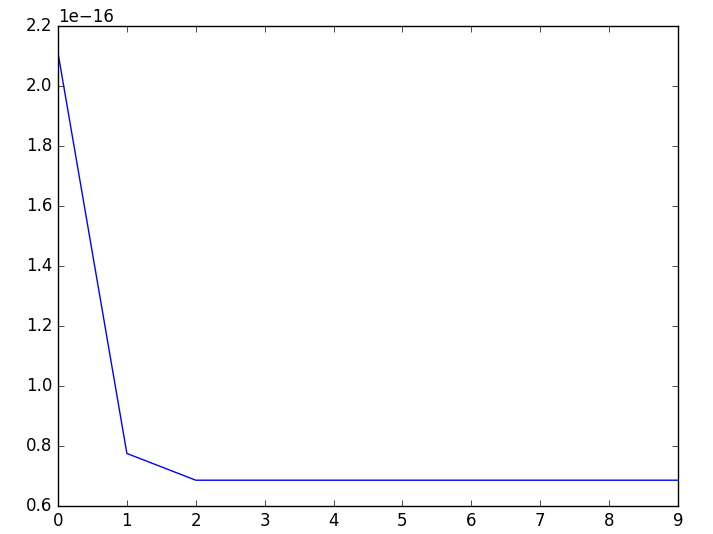
\includegraphics[width=\textwidth,height=\textheight,keepaspectratio]{iterative_refinement_crop}
\caption{Итерационное уточнение постоянной точности для систем вида $Ax=b$. Ось x - количество итераций, ось y – значение отношения нормы вектора невязки $r$ к норме вектора $b$, равное  $||r||_{\infty} / ||b||_{\infty}$}
\end{figure}

Итерационное уточнение переменной точности показало значительное повышение точности решения при аналогичных параметрах тестирования (в данном случае выполнялась лишь одна итерация). Для одинарной точности использовалась арифметика 32-битных чисел с плавающей запятой. Среднее относительное отклонение составило 2.0171e-16 при использовании переменной точности, тогда как при постоянной точности был получен результат, равный 1.1922e-09.

%%%%%%%%%%%%%%%%%%%%%%%%%%%%%%%%%%%%%%%%%%%%%%%%%%%%%%%%%%%%%%%%%

\subsection{Оценщик числа обусловленности}
Был реализован оценщик числа обусловленности матрицы системы в строчной норме. На графике 2 изображены точные и оцененные значения числа обусловленности для случайных матриц, заполненных случайными числами, а на графике 3 - для случайных матриц, являющимися почти сингулярными. 
Необходимо уточнить, что используемый нами алгоритм генерации почти сингулярных матриц с некоторой вероятностью способен создать и недостаточно плохо обусловленную матрицу, чем можно объяснить наличие "провалов" на последнем графике. 

Стоит отметить, что построенный оценщик соответствует требованию, суть которого заключается в том, что оценка числа обусловленности не должна превышать точно вычисленное значение. Данное требование лежит в основе подхода реализованного алгоритма. Также стоит отметить тот факт, что алгоритм устойчиво выдаёт оценку, имеющую отклонение от точного значения не более чем на 1-1.5 порядка, что наглядно продемонстрировано на графике 3. 

\begin{figure}[ht]
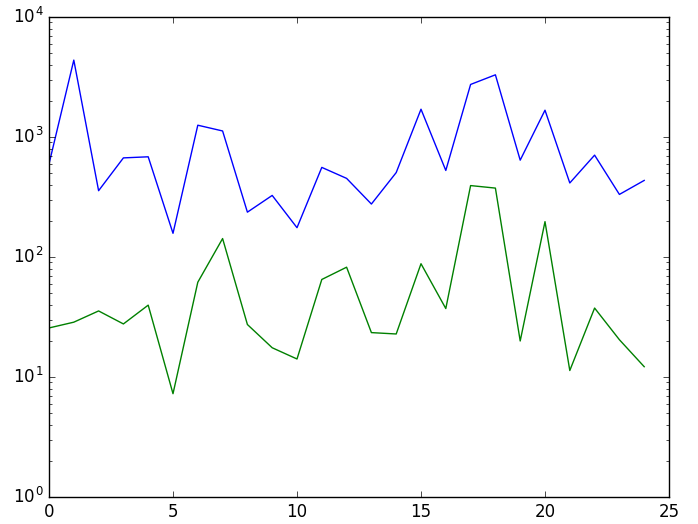
\includegraphics[width=\textwidth,height=\textheight,keepaspectratio]{figure_2_cropped}
\caption{Оценка числа обусловленности для случайных матриц. Ось x - номер теста, ось y - значение числа обусловленности. Синим цветом обозначены точные значения числа обусловленности, зелёным – найденная оценка. }
\end{figure}

\begin{figure}[ht]
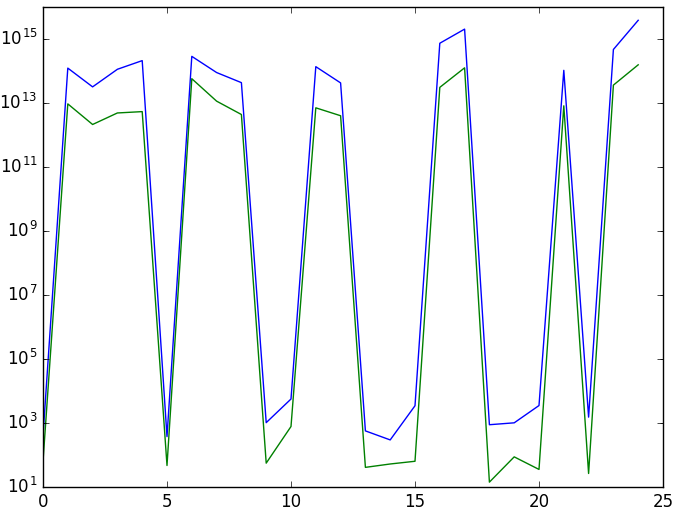
\includegraphics[width=\textwidth,height=\textheight,keepaspectratio]{figure_4_cropped}
\caption{Оценка числа обусловленности для матриц, близких к сингулярным. Ось x - номер теста, ось y - значение числа обусловленности. Синим цветом обозначены точные значения числа обусловленности, зелёным – найденная оценка.}
\end{figure}


